% Typeset with LaTeX format
% Using AMS extensions for mathematical formatting

%	The 'myarticle' class gives me a smaller title size
%	This class should appear as 'article'
%	in any submitted source file, so that others can
%	properly format it.  Please change if it is not correct.
%  	I use the 'leqno' option, for left-handed equation numbers.
\documentclass[leqno,12pt]{article}
%	To get all the formal devices, I usually use
%	all of 'amsmath', 'amssymb', and 'amsthm'.
%	There may also appear the packages
%	'setspace' (for double-spacing)
%	and 'mylogic' (for personal margins, headers, commands, etc.)
%	These should NOT appear in any submitted source file.
%	Please remove them if still here upon submission.
\usepackage{amsmath,amssymb,amsthm,amscd,amsxtra,latexsym}
\usepackage{notation}
\usepackage{enumerate}
\usepackage{url}
\usepackage{color}
\usepackage{graphicx}


%---------------------------------------------
%       OPTIONAL:  PAGE SPACING HERE
%---------------------------------------------

\usepackage{setspace}
%	The following line may be commented out
% 	If so, it can be deleted without affecting anything.
%	I use the command (with the 'setspace.sty' package)
%	for alternative formatting (also \doublespacing).
%	If this line is commented out, and 'setspace' is not in use,
%	the document formats as usual for its class.
\doublespacing

%---------------------------------------------
%       PAGE FORMAT (BORDERS/HEADERS)
%---------------------------------------------

%	Page format commands:
%	Override normal article margins,
%	making the margins smaller
\setlength{\textwidth}{6.5in}
\setlength{\textheight}{8.5in}
\setlength{\oddsidemargin}{0in}
\setlength{\evensidemargin}{0in}
\setlength{\topmargin}{0in}

%	More format:
%	Adds my name, date of compiling/printing
%	to header, small text 
%	(page #'s also appear in head)
\pagestyle{myheadings}
\markright{\footnotesize M. Allen---DeepDream (CS 135)}
\thispagestyle{empty}

%---------------------------------------------
%       DEFINED COMMANDS
%---------------------------------------------

%---------------------------------------------
%       DOC STARTS HERE
%---------------------------------------------

\begin{document}

\begin{center}
\singlespacing
{\bf 
	Daydream Believer: Google's DeepDream Project\\
	Marty Allen \\
	Introduction to Machine Learning (CS 135)
}

\vspace{18pt}
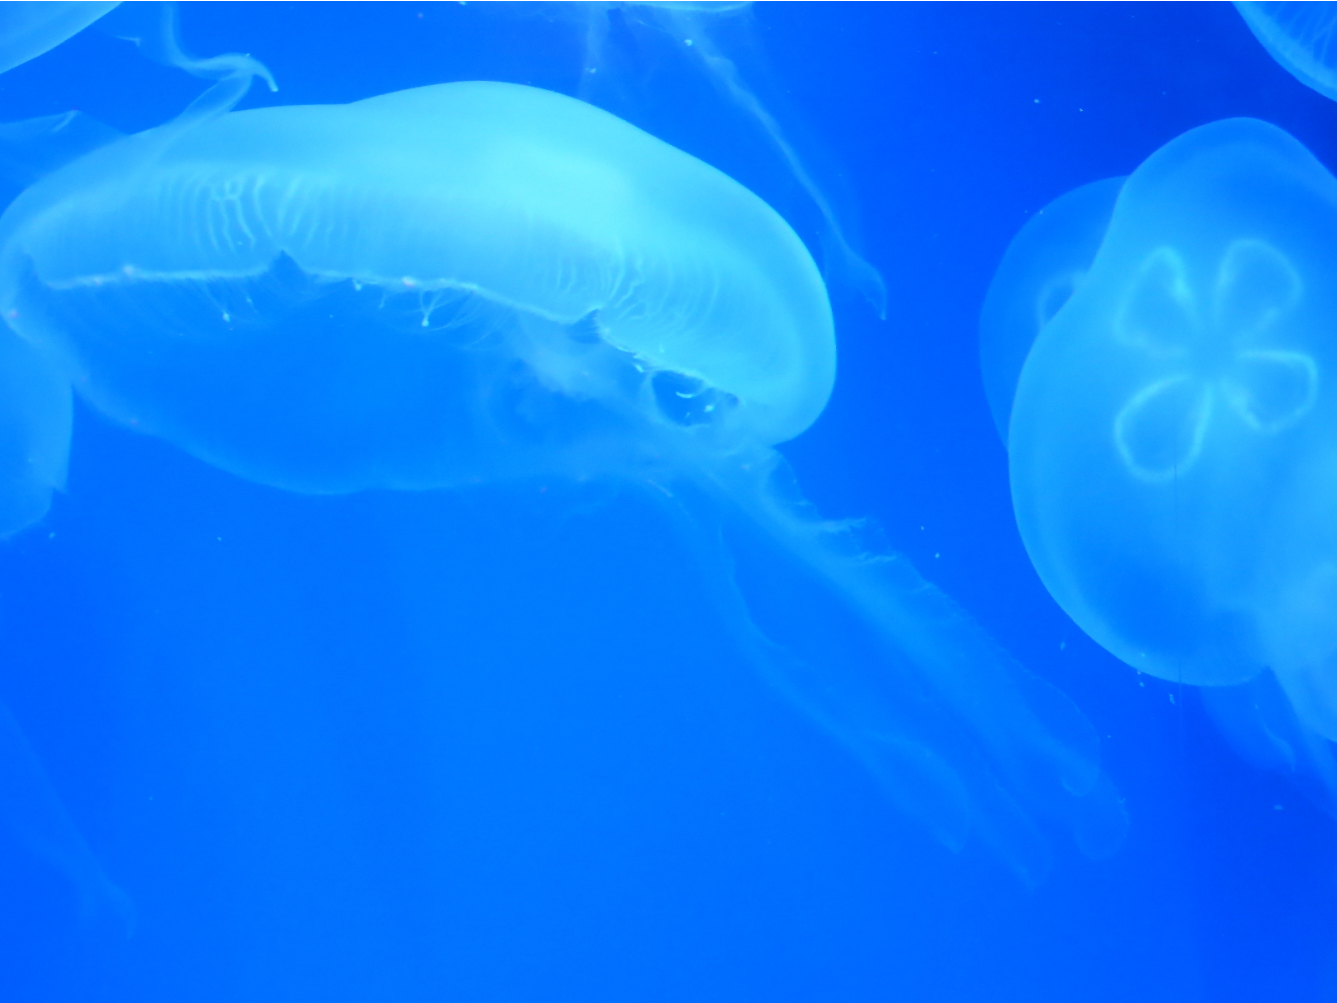
\includegraphics[width=3in]{fish} \vspace*{.5in}
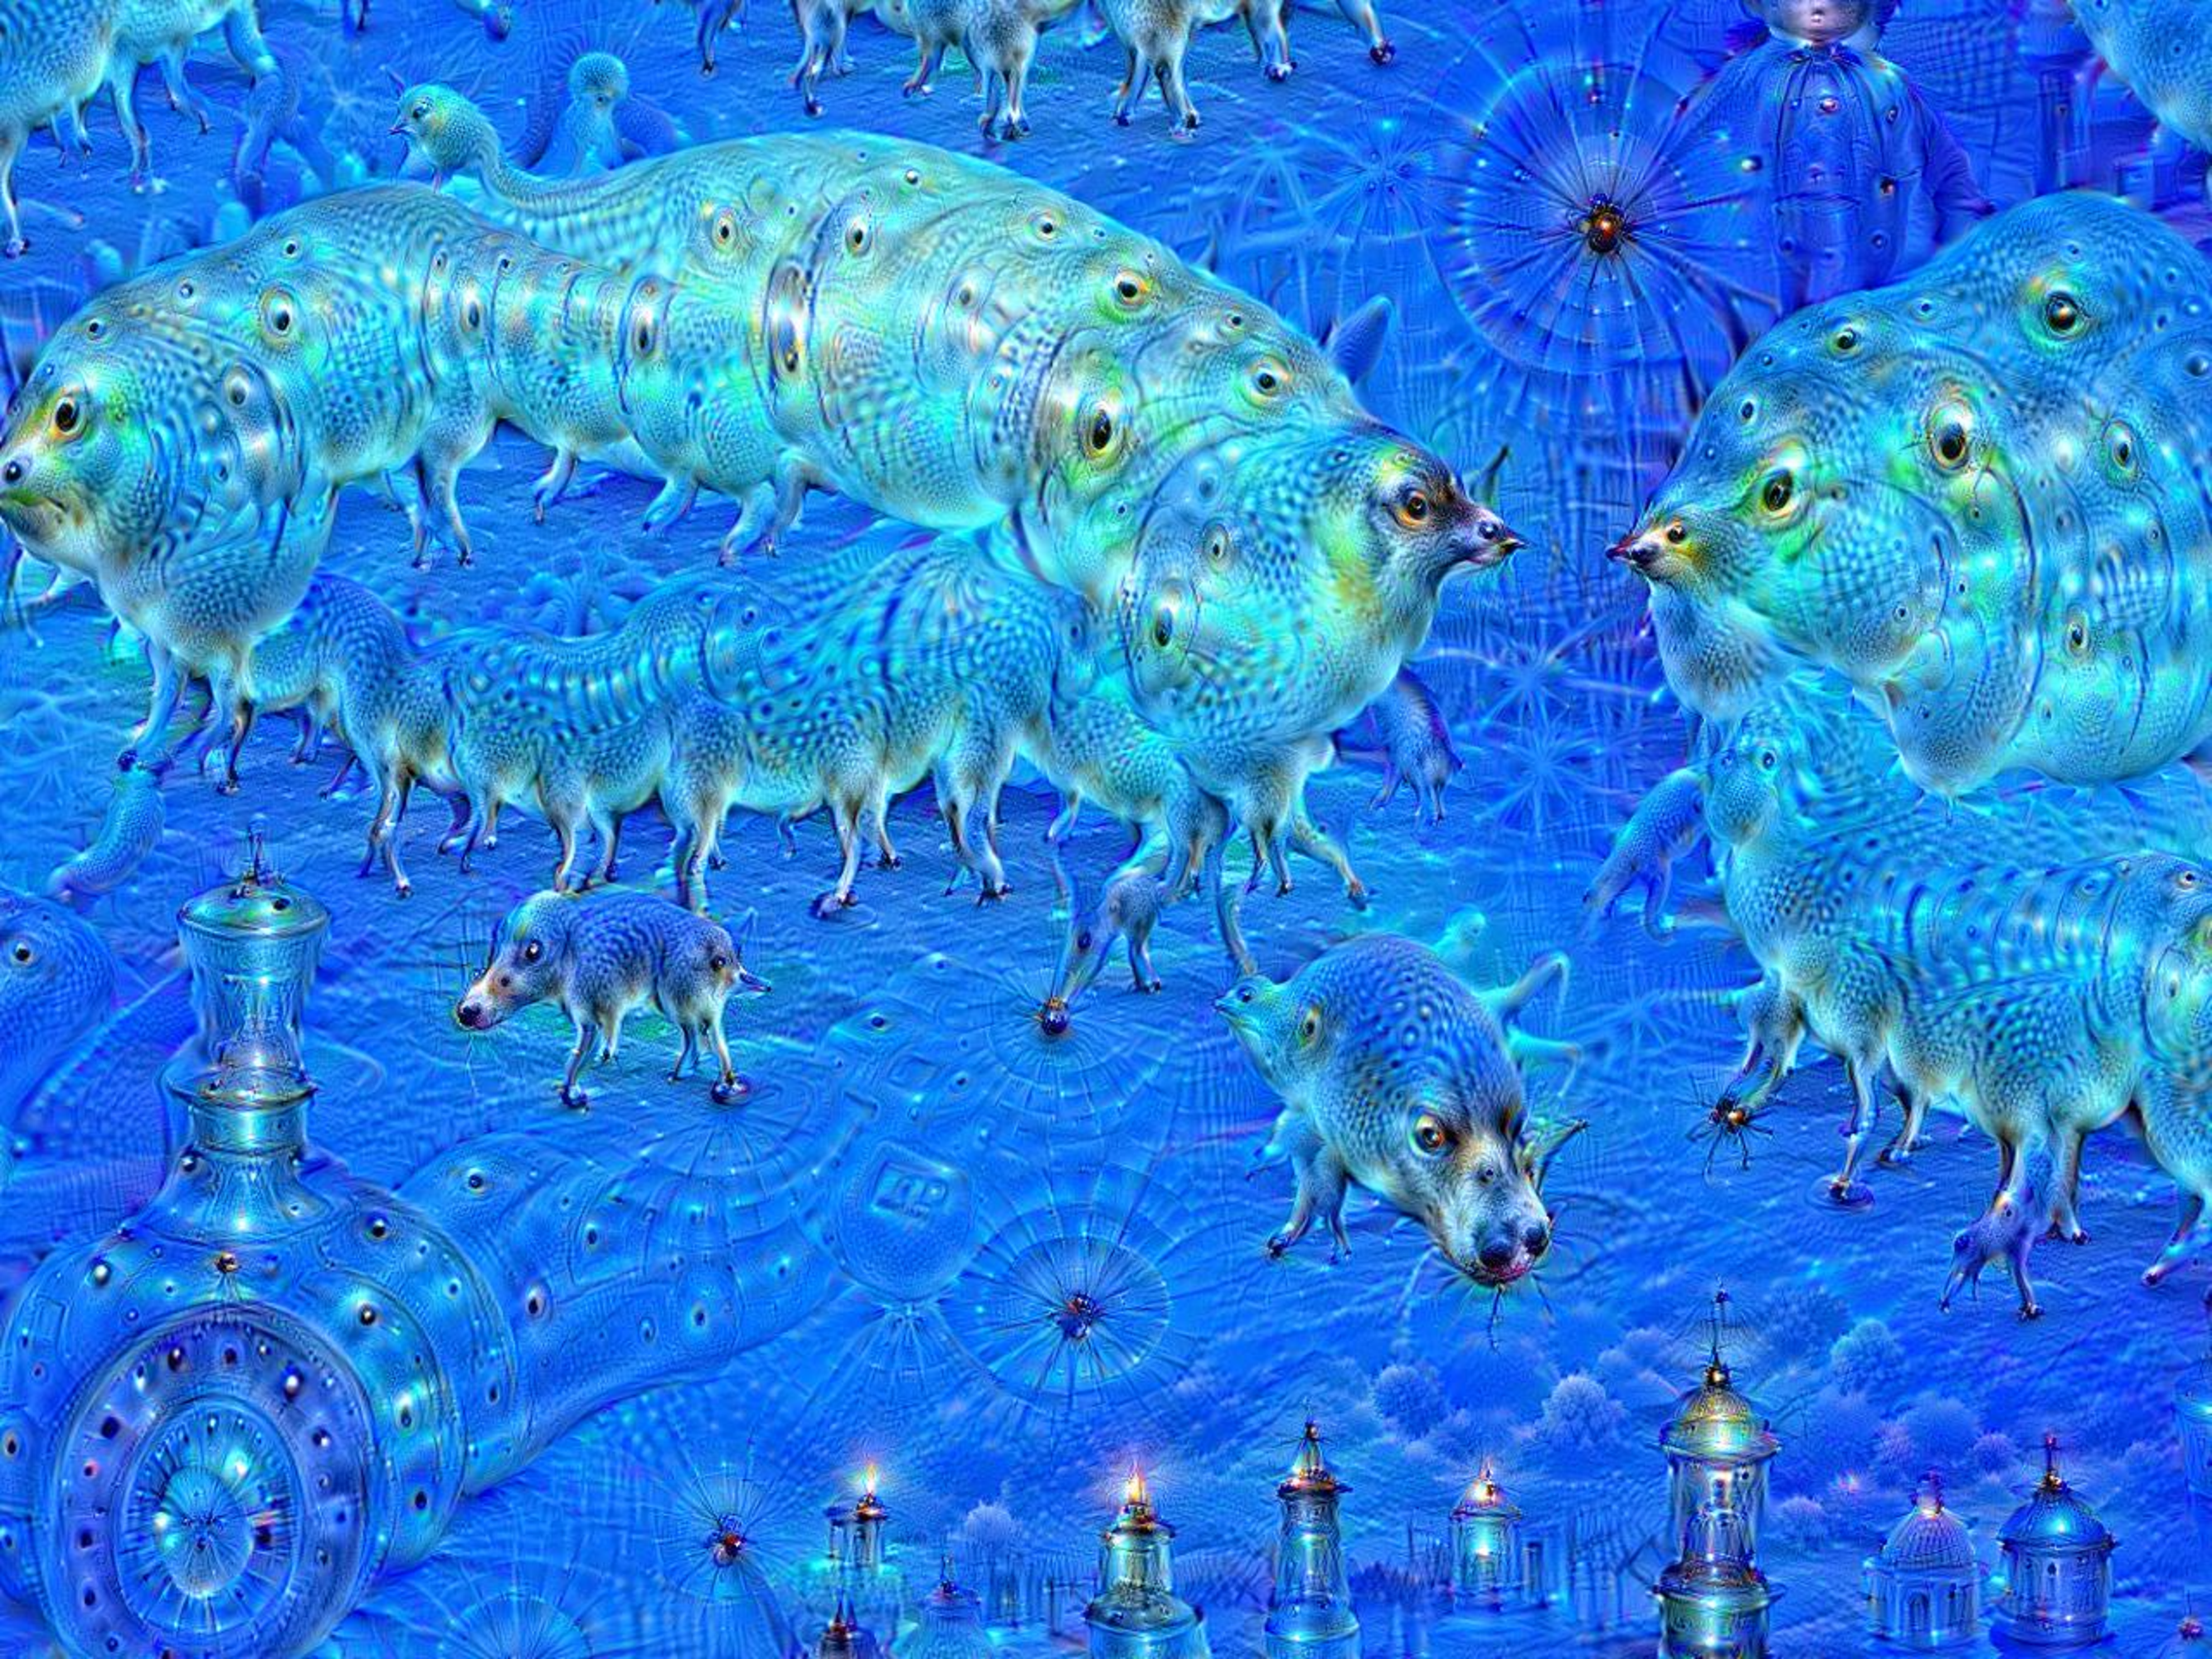
\includegraphics[width=3in]{deepDreamFish}
\end{center}

\vspace{-0.5in}

\doublespacing
\noindent 
DeepDream is a program primarily designed by Google software engineer Alexander Mordvintsev, and designed to
``reverse'' the process by which a neural network is trained to recognize images \cite{deepdreamsite}.
The images above are an example of what the program produces.\footnote{Images by Martin Thoma, 
(Wikipedia), Creative Commons CC0 1.0 Universal Public Domain licensing.}  On the left is a photo of some
jellyfish;  on the right is the result of applying DeepDream to that image, using a ``deep'' network---that is,
a \emph{convolutional neural network}---that had originally been trained to recognize images containing such
things as dogs, children, and buildings.  The result is a phantasmagorical transformation of the image, where the
jellyfish appear to be made up out of conglomerations of dogs, birds, and perhaps insects, and the water itself
is a cascade of semi-organic buildings and swirling shapes, including what appears to be a single child in the
upper-right background.

While DeepDream itself is meant as merely a curiosity, allowing users to generate their own strange and surreal
images from whatever source they choose, it is based upon techniques and concepts of some importance in neural network
research.  As we learned in class, a standard \emph{feed-forward} neural network is composed of one or more
layers of ``neurons'' joined together in a graph structure \cite[\S18.7]{RussellNorvig10}.  The first
layer of the network receives the \emph{inputs} to the network, a set of numerical features that characterize a
piece of data.  The last layer in the network generates its \emph{outputs}. In between, there may be one or more
\emph{hidden layers}, each of which consists of neurons that connect the layers above and below it.  Typically,
each neuron in any layer after the first input layer connects back to each of the neurons in the layer before
it.  For each such connection, the neuron stores a \emph{weight}, $w$.  When the network is in use, values are
passed in to its first layer.  Each neuron at the next layer then takes all of these input parameter values,
$\seq{a_1,\, a_2,\, \ldots,\, a_n}$ and computes the weighted sum over all these values, before applying some
function, $g$, to that weighted sum.  The result of this process is then the value which the neuron passes along
to the neurons in the next layer down, which repeat the process all the way to the last layer.  

The outputs of a neural net are thus vectors of values, one per neuron in the final layer.  Typically, if the
network is being used for a \emph{classification} problem---where it is categorizing the \emph{type} of thing
the input represents---there will be one output neuron for each class of entity, and the final classification
will be that one represented by the output neuron whose final value is the largest.  In a single-object image
classification problem where we are trying to classify images into pictures containing a human face and pictures
that do not contain a face, for instance, inputs to the network might consist of pixel values of images, and
there would be a 2-neuron output layer, where the first neuron might represent the presence of a face, and the
second might represent the absence of a face.

In order to produce networks that can actually do this sort of classification, we usually start with a
\emph{training set} of known data, say images for which we already know whether or not they contain faces.
The network is initially set to apply merely random weights on all its connections, and is then trained to
minimize output error---the average difference between what the network \emph{says} each image contains and what
we \emph{already know} they contain.  This training can be handled via a process of \emph{backpropagation},
where a program repeatedly computes the results for images in the training set by moving forward from input
neurons to output neurons, measuring the error in each case, and then adjusting the weights backward from output
neurons to the first hidden layer, repeating until overall error is minimized.  This technique, first developed
in control theory in the early 1960's, was popularized for use in neural networks in the 1980's
\cite{Dreyfus90,Rumelhart86}.  Recent computing advances have made the idea much more practical as modern
processors, including graphics processing units (GPU's) and custom-built chips, can handle backpropagation for
larger and more complex networks than were previously feasible.

The convolutional neural networks used in DeepDream date to work from the 1990's \cite{LeCun98}.  In such
networks, multiple layers of networks, some operating in parallel, and some in series, are used to extract
classification data from inputs.  Unlike traditional networks, however, less attention is paid to
hand-engineering features of the data, and more to the structure of the network, which itself settles on
features through a multi-step process of refinement and abstraction.  The process of learning with such complex
networks---now popularly known as \emph{deep learning}---has been made possible by further advances in both
computing hardware and algorithms for efficiently training on massive data-sets \cite{Goodfellow16,Hinton06}.

DeepDream started as a deep learning convolutional neural network for classifying the content of complex images.
Fed with massive data-sets of images and associated information, the network was trained to be able to recognize
a wide range of different objects in image data.  However, once this process was complete, many things remained
unknown.  Indeed, it is a common feature of neural networks, especially the highly complex convolutional ones
used in deep learning, that we often do not know \emph{what} features the network is actually trained to
recognize.  While we may suspect that some layers of a convolutional network train themselves to recognize
edges, while others train to recognize colors or textures, we usually cannot be sure.  This can make future
behavior of networks somewhat hard to predict, which can lead to uncertainty about outcome quality over time.
As Olah, \emph{et al}.\ write in a recent review of the visualization techniques used in the DeepDream project,
``a growing sense [exists] that neural networks need to be interpretable to humans'' \cite{Olah17}.

The visualization capabilities of DeepDream are based on this idea.  The original concept dates back to the
1980's, in application to simpler feed-forward networks \cite{Lewis88}, but has been more recently extended to
deep networks \cite{Erhan09,Olah17}.  In this approach, once a network is trained, we can begin to discern what
one of its layers actually responds to by creating \emph{synthetic data} that is specifically optimized to
cause neurons in that layer to activate.  That is, we begin with an existing image (often a randomly generated
collection of pixel values) and then determine the overall activation pattern generated for the neurons in the
layer of interest.  Using a method related to backpropagation, we then ``reverse'' the functions used on inputs
to that neuron---technically taking the derivatives of those functions---to compute back to the image itself.
However, unlike in normal backpropagation, which was used in training the network in the first place, we
\emph{do not} modify weights in the network.  Instead, we use the reversed function to compute changes in the
\emph{input values} themselves, actually modifying the image pixel values repetitively to get the highest
overall rate of response from the neurons at our intermediate layer.

As Olah \emph{et al}.\ point out, however, a simple-minded application of this process usually produces nothing
of real interest. The problem being solved is one of \emph{optimization}: we seek to find the \emph{best}
images, understood as those that make a layer of neurons as ``excited'' as possible.  As it turns out, in most
cases, the best possible images for such a purpose do not resemble the real-world ones on which we train the
networks in the first place.  Instead ``you end up with a kind of neural network optical illusion---an image
full of noise and nonsensical high-frequency patterns,'' a form of random visual static \cite{Olah17}.  To
combat this, and generate images with features that we ourselves may be able to recognize, a process of
\emph{regularization} is applied as the synthetic images are modified to optimize neural layer response.  A
variety of approaches can be applied, but in each case it amounts to modifying the optimization process so that
we measure success as a combination of the amount to which the image make the neural layer respond, as well as 
other measures having to do with features of the resulting synthetic image itself.  For example, we might
penalize images for which neighboring neurons have high variance, subtracting the amount of this variance from
the measure of layer response, and seeking images that have the best balance between the two, therefore
preferring less-noisy images overall \cite{mahendran15}.  

Carefully handled, such a process zeroes in on recognizable features that a network layer is responding to, and
``separates the things causing behavior from things that merely correlate with the causes'' \cite{Olah17}. By
generating multiple diverse images and comparing them, we can better intuit what a layer is ``looking for.''
Again, the desire for diversity can be added to the function that computes how good a synthetic image is for
visualization purposes, with each image that is generated rated based on a combination of:
\begin{enumerate} \cutwspace
	\item How actively the layer we are interested in responds to the image, with higher response levels
		corresponding to a \emph{higher-rated} image.
	\item How irregular and noisy the image is, with high irregularity \emph{reducing} the overall
		rating of the image.
	\item How similar the image is to others we have already generated, with high similarity also
		\emph{reducing} the image's overall rating.
\end{enumerate}
Combining all of these together, it is possible to automatically generate images that contain visual features
that are recognizable to human beings, while also being different enough to compare.  Based on a single example
of a synthetic image, identifying its salient features may be quite difficult:  we may not know whether it is
the set of edges of the shapes in the image that is being responded to, or the color and texture of the image or
some combination of those features.  With multiple examples, however, these differences may become more clear.
If we see that our images all have different colors and textures, but all feature similar curves and lines, then
we can start to understand that the neuron layer we are examining is meant to respond to the curves and lines
(presumably color and texture are either unimportant for the classification task at hand, or are handled by
other layers of the network).

In DeepDream, the final piece of the puzzle is to dispense with the completely synthetic nature of the data.
Rather than starting with random pixel values, and optimizing to recognizable features, we start with an
existing image, and modify it progressively so that it causes our layer to respond more strongly, while
maintaining regularity as much as possible to avoid noisiness, and stopping when we have modified it only a
relatively small amount from the original source data.  The result is the sort of strange combination seen in
the example images with which we started:  a mix of overall shapes that resembles the original composition of
the scene, but tweaked in ways that optimize the responses of layers meant to recognize particular things not
actually found in the image at all.  Done using the first layer or two of a convolutional network, the results
are actually as expected---we often see that earlier layers respond to things like edges, and the results of
doing the backwards optimization merely sharpens edges and gaps in the image.  As researchers have found,
however, the deeper convolutional layers of these complex classification networks build up subtle responses to
complex image features, responding to things we can optically identify as plants, animals, buildings, etc.
Thus, when we apply the optimization process to those sorts of layers, the original image is turned
into a hallucinatory pastiche of these sorts of objects as pixels are tweaked from their original values into
combinations of the source image and parts of the ones that formed the original training data.


\pagebreak

\singlespacing

\bibliographystyle{plain}
 \bibliography{./sample_essay}



\end{document}
 
